% Based on the DML course template (https://github.com/dml-cth/deep-machine-learning/tree/master/poster-template),
% adapted from https://github.com/deselaers/latex-beamerposter/blob/master/examples/03/poster.tex
% Build: poster/build.ps1 (pdflatex, bibtex, pdflatex, pdflatex).
% Figures, screenshots and the numbers in fig/results.tex: python poster/make_figures.py (repository root);
% new screenshots: python poster/capture_combos.py models/fox_rl_3h.pt


\documentclass{beamer}
\usepackage[orientation=portrait,size=a2,scale=1.3,debug]{beamerposter}
\mode<presentation>{\usetheme{ZH}}
\usepackage{chemformula}
\usepackage[utf8]{inputenc}
\usepackage[german, english]{babel} % required for rendering German special characters
\usepackage{siunitx} %pretty measurement unit rendering
\usepackage{hyperref} %enable hyperlink for urls
\usepackage{ragged2e}
\usepackage[font=scriptsize,justification=justified]{caption}
\usepackage{array,booktabs,tabularx}
\usepackage{tikz}
\usetikzlibrary{arrows.meta,positioning}
\usepackage{multicol}

% Replacement font for Akzidenz
\usepackage{helvet}

\newcolumntype{Z}{>{\centering\arraybackslash}X} % centered tabularx columns

% The two policies keep the same colours in every figure.
\definecolor{bcblue}{HTML}{2A78D6}
\definecolor{rlorange}{HTML}{EB6834}
\newcommand{\KL}{\mathrm{KL}}
% Written by poster/make_figures.py: numbers the poster text uses.
\newcommand{\rlHours}{3}
\newcommand{\cpuGames}{20}
\newcommand{\ganonGames}{20}
\newcommand{\vsGames}{40}
\newcommand{\cpuBC}{95\% \;(+2.2)}
\newcommand{\cpuRL}{100\% \;(+3.0)}
\newcommand{\ganonBC}{65\% \;(+0.5)}
\newcommand{\ganonRL}{95\% \;(+2.0)}
\newcommand{\vsRL}{62\% \;(+0.7)}
\newcommand{\cpuRLwin}{100\%}
\newcommand{\ganonRLwin}{95\%}
\newcommand{\cpuBCwin}{95\%}
\newcommand{\ganonBCwin}{65\%}
\newcommand{\vsRLwin}{62\%}
\newcommand{\sdHuman}{7\%}
\newcommand{\sdBC}{17\%}
\newcommand{\sdRL}{6\%}
\newcommand{\comboBC}{2.67}
\newcommand{\comboRL}{2.35}
\newcommand{\klLevel}{0.03}
\newcommand{\lcancel}{86--89\%}
\newcommand{\styleSpread}{11\%}
\newcommand{\fps}{550}
\newcommand{\humanPlayers}{22}
 % results, written by make_figures.py

% A headline result: big number, what it is, comparison.
\newcommand{\stattile}[3]{%
	\begin{tikzpicture}
		\node[draw=rlorange, line width=2.5pt, fill=rlorange!10, rounded corners=10pt, text width=5.1cm,
			minimum height=3.3cm, align=center, inner sep=6pt]
			{{\Huge\bfseries\color{rlorange}#1}\\[8pt]{\small\bfseries #2}\\[3pt]{\footnotesize\color{black!65}#3}};
	\end{tikzpicture}}

\title{\huge Combos, Not Spam: A Human-Like\\ Super Smash Bros.\ Melee Bot}
\author{Your Name, Teammate Name}
\institute[Chalmers]{Chalmers University of Technology \\ Electrical Engineering Department}
\date{\today}

% edit this depending on how tall your header is.
\newlength{\columnheight}
\setlength{\columnheight}{50cm}


\begin{document}
\begin{frame}
\begin{columns}
	\begin{column}{.5\textwidth}
		\begin{beamercolorbox}[center]{postercolumn}
			\begin{minipage}{.98\textwidth}  % tweaks the width, makes a new \textwidth
				\parbox[t][\columnheight]{\textwidth}{
					\begin{myblock}{Motivation}
						\begin{center}
							{\large\bfseries\color{ETH3} Can a bot learn to \textcolor{rlorange}{combo} instead of spam?}
						\end{center}
						\begin{figure}
							\centering
							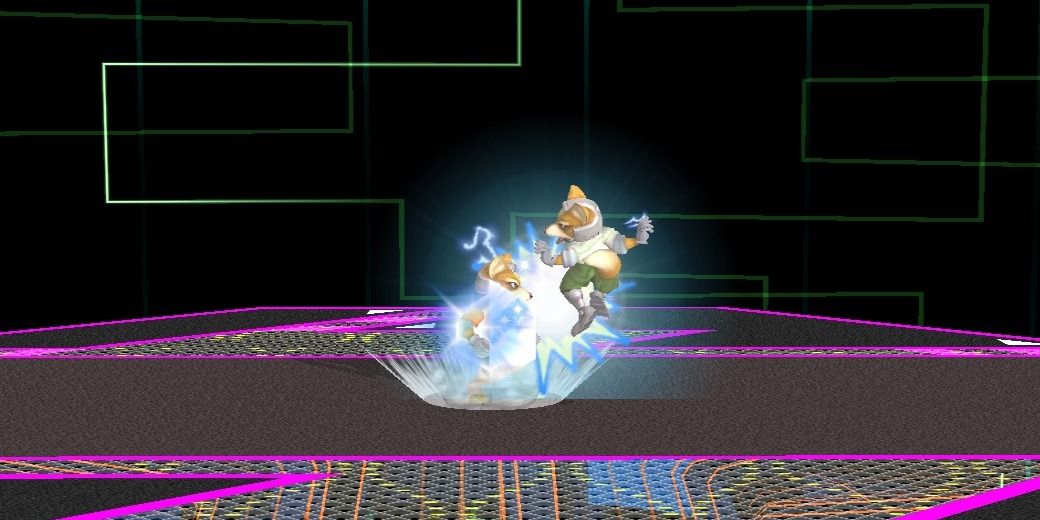
\includegraphics[width=\linewidth]{fig/hero.jpg}
							\caption{Our bot (left) ends a forward-air $\rightarrow$ drill $\rightarrow$ shine combo
							on the level 9 CPU: Fox's signature combo, captured from the emulator.}
						\end{figure}
						\begin{itemize}
							\item \textbf{Melee}: 60 frames/s, frame-precise technique. Deep RL has beaten pros
							\cite{firoiu2017}, but our first PPO bot won by \textbf{spamming one move}.
							\item \textbf{Goal}: a Fox that is strong \emph{and} plays like a human.
						\end{itemize}
					\end{myblock}\vfill
					\begin{myblock}{Problem formulation}
						\begin{itemize}
							\item \textbf{Observe} $h_t$: both players' position, speed, damage, action state, \dots
							\item \textbf{Act} $a_t$: a full controller per frame, $48 \cdot 17 \cdot 17 \cdot 5
							\approx 69$k choices (buttons, stick $x$, $y$, C-stick).
							\item \textbf{React like a human} \cite{firoiu2018}: 18 frames (300\,ms) late.
						\end{itemize}
						\begin{center}
							\begin{tikzpicture}[x=0.82cm, y=1cm]
								\draw[line width=2pt, ETH3!60] (0,0) -- (19.5,0);
								\foreach \i in {0,...,19} {\draw[line width=1.5pt, ETH3!60] (\i,-0.18) -- (\i,0.18);}
								\fill[bcblue] (0,0) circle (0.28);
								\fill[rlorange] (18,0) circle (0.28);
								\node[below=4pt, font=\small] at (0,-0.15) {see frame $t$};
								\node[below=4pt, font=\small] at (18,-0.15) {press at $t+18$};
								\draw[-{Latex[length=14pt]}, line width=2.5pt, ETH3] (0.3,0.4) to[bend left=12]
									node[above, font=\small] {decision waits 18 frames} (17.7,0.4);
							\end{tikzpicture}
						\end{center}
						\textbf{Objective}: win, but stay close to how humans play:
						\begin{equation*}
							\max_\theta\; \mathbb{E}_{\pi_\theta}\Big[\sum_t \gamma^t r_t\Big]
							- \beta \sum_t \KL\big(\pi_\theta(\cdot \mid h_t)\,\big\|\,\pi_{\text{human}}(\cdot \mid h_t)\big)
						\end{equation*}
					\end{myblock}\vfill
					\begin{myblock}{Method: two phases}
						\begin{center}
							\begin{tikzpicture}[
									box/.style={draw=ETH3, line width=2pt, rounded corners=8pt, align=center,
										inner sep=8pt, font=\small, minimum height=2.2cm},
									arr/.style={-{Latex[length=16pt]}, line width=3pt, ETH3}]
								\node[box, fill=white, text width=3.8cm] (data) {Human replays\\[2pt]111k games};
								\node[box, fill=bcblue!18, text width=3.8cm, right=2.0cm of data] (bc)
									{Imitation\\[2pt]policy $\pi_{\text{BC}}$};
								\node[box, fill=rlorange!18, text width=3.8cm, right=2.0cm of bc] (rl)
									{RL policy\\[2pt]$\pi_\theta$};
								\draw[arr] (data) -- node[above, font=\footnotesize] {Phase 1} (bc);
								\draw[arr] (bc) -- node[above, font=\footnotesize] {Phase 2} (rl);
								\node[box, fill=tlg!50, text width=15cm, minimum height=1.2cm, below=0.9cm of bc,
									xshift=1.5cm] (opp)
									{opponents: past versions of itself $\cdot$ Ganondorf PPO bot $\cdot$ CPU 9};
								\draw[arr] (opp.north -| rl) -- node[right, font=\footnotesize] {self-play} (rl.south);
								\draw[-{Latex[length=16pt]}, line width=3pt, bcblue, dashed]
									(bc.north) to[bend left=30] node[above, font=\footnotesize, text=bcblue]
									{start + KL leash} (rl.north);
							\end{tikzpicture}
						\end{center}
					\end{myblock}\vfill
					\begin{myblock}{Phase 1: learning from humans}
						\begin{columns}[T]
							\begin{column}{0.56\textwidth}
								\begin{itemize}
									\item \textbf{Data}: 111,310 ranked games of master and diamond Fox players
									\cite{dataset}, 1.24 billion frames.
									\item \textbf{Policy}: 3 $\times$ (residual LSTM \cite{lstm} + MLP), width 512,
									autoregressive heads; 9.9\,M parameters, as in slippi-ai \cite{slippiai}.
								\end{itemize}
							\end{column}
							\begin{column}{0.42\textwidth}
								\begin{figure}
									\centering
									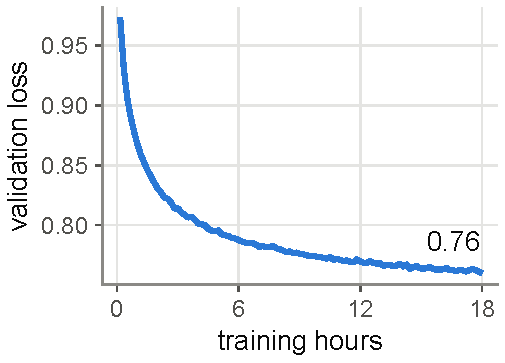
\includegraphics[width=\linewidth]{fig/imitation_loss.pdf}
									\caption{18 h on one laptop GPU. Accuracy: buttons 93\%, sticks 89/94\%,
									C-stick 99\%.}
								\end{figure}
							\end{column}
						\end{columns}
						\textbf{Behaviour cloning}: predict the human's controller 18 frames ahead:
						\begin{equation*}
							\mathcal{L}_{\text{BC}}(\theta) = -\sum_t \sum_{k=1}^{4}
							\log \pi_\theta\big(a^{(k)}_{t+18} \,\big|\, h_{t},\, a^{(<k)}_{t+18}\big)
						\end{equation*}
					\end{myblock}\vfill
		}\end{minipage}\end{beamercolorbox}
	\end{column}
	\begin{column}{.5\textwidth}
		\begin{beamercolorbox}[center]{postercolumn}
			\begin{minipage}{.98\textwidth} % tweaks the width, makes a new \textwidth
				\parbox[t][\columnheight]{\textwidth}{
					\begin{myblock}{Phase 2: reinforcement learning on a leash}
						PPO \cite{ppo} + a KL penalty to the frozen imitation policy \cite{seqtutor,alphastar}:
						\begin{equation*}
							\mathcal{L}(\theta) = \mathbb{E}_t\Big[-\min\big(\rho_t \hat{A}_t,\,
							\mathrm{clip}(\rho_t, 1 \pm \epsilon)\,\hat{A}_t\big)
							+ \beta\, \KL\big(\pi_\theta \,\|\, \pi_{\text{BC}}\big)(h_t)\Big]
						\end{equation*}
						\begin{equation*}
							r_t = \Delta \text{stocks}_{\text{opp}} - \Delta \text{stocks}_{\text{own}}
							+ 0.01\,\big(\Delta\%_{\text{opp}} - \Delta\%_{\text{own}}\big) + r_t^{\text{shape}}
						\end{equation*}
						\begin{itemize}
							\item $r_t^{\text{shape}}$: small anti-exploit terms; GAE \cite{gae}, $\gamma = 0.997$,
							$\beta = 0.5$, $\epsilon = 0.2$.
							\item 10 parallel games (libmelee \cite{libmelee}): 6 self-play, 2 Ganondorf, 2 CPU 9.
						\end{itemize}
					\end{myblock}\vfill
					\begin{myblock}{Results: win rates after \rlHours{} h of RL}
						\begin{center}
							\stattile{\cpuRLwin}{vs CPU level 9}{imitation: \cpuBCwin}\hfill
							\stattile{\ganonRLwin}{vs Ganondorf bot}{imitation: \ganonBCwin}\hfill
							\stattile{\vsRLwin}{vs imitation}{its own teacher}
						\end{center}
						\begin{figure}
							\centering
							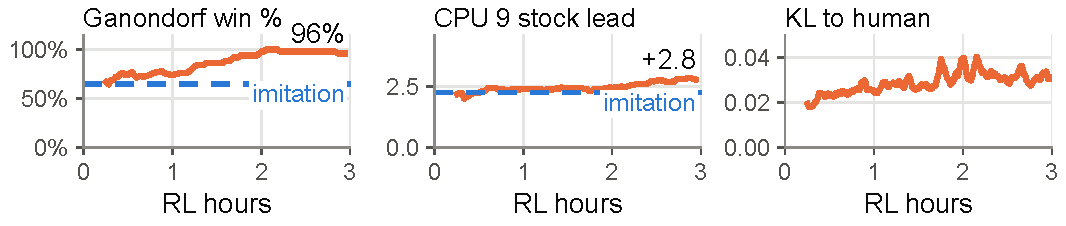
\includegraphics[width=\linewidth]{fig/rl_curves.pdf}
							\caption{During RL: rolling mean over 50 games (dashed: imitation). The distance to the
							human policy levels off at \klLevel{} nats/frame. Final Destination, 4 stocks,
							\cpuGames--\vsGames{} games per test.}
						\end{figure}
					\end{myblock}\vfill
					\begin{myblock}{Results: still human-like}
						\begin{figure}
							\centering
							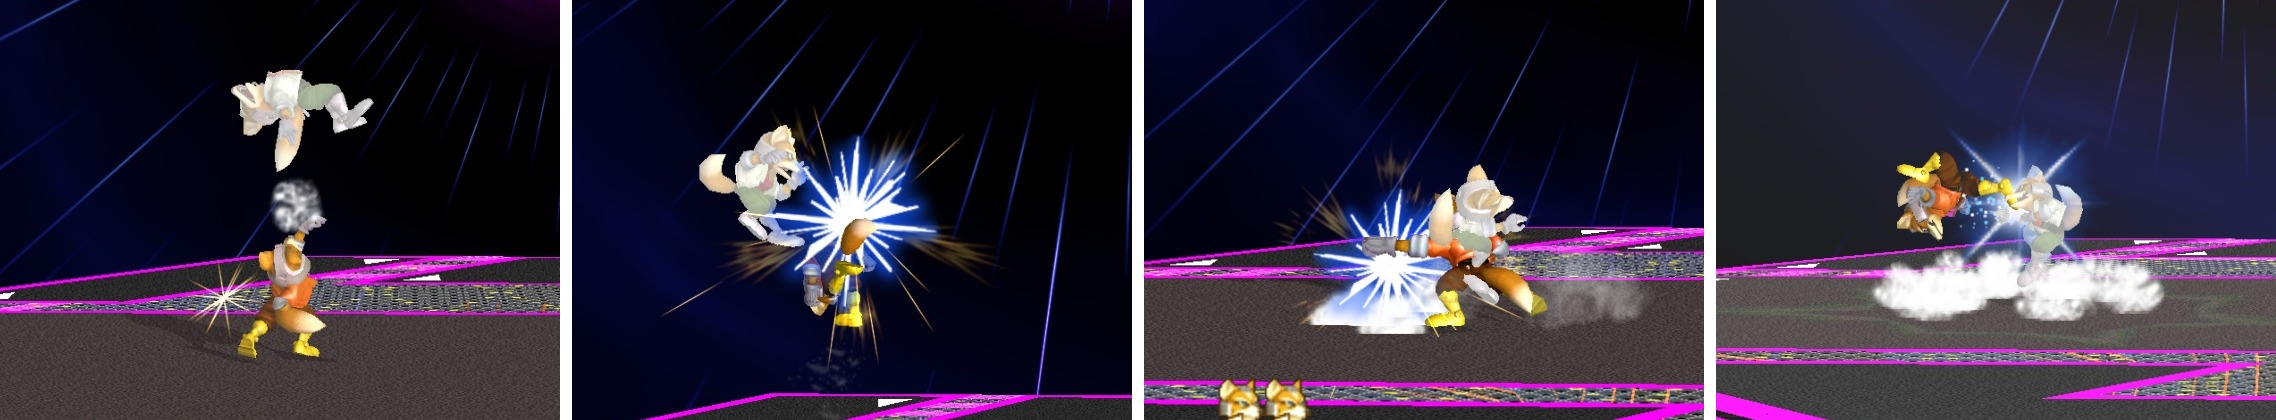
\includegraphics[width=\linewidth]{fig/combo_strip.jpg}\\[4pt]
							% Written by poster/make_figures.py: labels under fig/combo_strip.jpg.
{\small\begin{tabularx}{\linewidth}{ZZZZ}
\textbf{1} up-throw {\color{black!55}127\%} & \textbf{2} up-air {\color{black!55}138\%} & \textbf{3} jab {\color{black!55}141\%} & \textbf{4} up-smash {\color{black!55}154\%}
\end{tabularx}}
\\[14pt]
							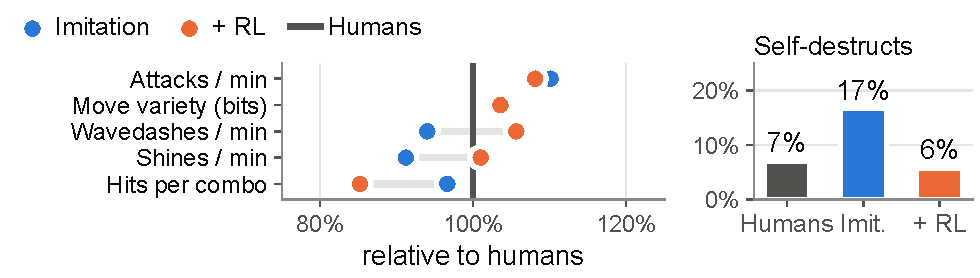
\includegraphics[width=\linewidth]{fig/style.pdf}
							\caption{Top: a combo by our bot, frame by frame, with the opponent's damage.
							Bottom: play style against \humanPlayers{} ranked human Fox players; self-destruct:
							a death without being hit in the 4\,s before.}
						\end{figure}
						\textbf{Self-destructs \sdBC{} $\rightarrow$ \sdRL} (humans \sdHuman); combos a bit shorter.
					\end{myblock}\vfill
					\begin{myblock}{Conclusion}
						\begin{itemize}
							\item Imitation gives human technique; RL on a KL leash adds wins, not spam.
							\item Next: all six stages, and games against people.
						\end{itemize}
					\end{myblock}\vfill
					\begin{myblock}{References}
						\scriptsize
						\begin{multicols}{2}
							\bibliographystyle{abbrv}
							\bibliography{./bib}
						\end{multicols}
					\end{myblock}\vfill
		}\end{minipage}\end{beamercolorbox}
	\end{column}
\end{columns}
\end{frame}
\end{document}
